\section{GUI}

\subsection{IndsætTitelHer}

Den grafiske brugerflade blev udviklet ved hjælp af QT, et program som er bygget op om C++ syntax, QT er brugervenligt og let at lære at skrive, hvis C++ allerede er et kendt programmeringssprog.\\
\subsection{Test}

Tekst
\begin{itemize}
	\item Tekst
	\item Tekst
	\item Tekst
\end{itemize}

\subsection{Test}

Tekst

\begin{itemize}
	\item Tekst
	\item Tekst
	\item Tekst

\end{itemize}


\subsection{Test}

Tekst

\begin{itemize}
	\item Tekst
	\item Tekst
	\item Tekst
\end{itemize}

Tekst


\subsection{Tidsplan}

\begin{figure}[h]
	\centering
		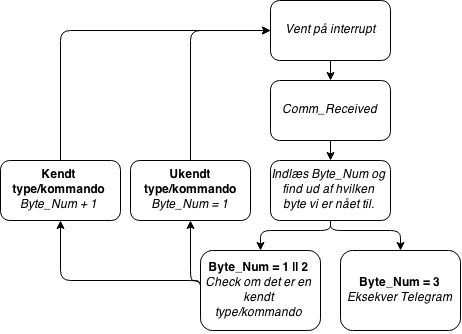
\includegraphics[scale=0.75]{Billeder/Comm_Modtagelse.png}
	\caption{Her kan vi se vores tidsplan}
	\label{fig:tidsplan}
\end{figure}